\chapter{Estado del arte}

% ------------------------------------------------------------------------------------------------------------

\section{Estimación de la edad en antropología forense}

\todo{Incluir gráfica con el número de publicaciones para estimación de la edad en antropología forense}

En ausencia de documentación escrita confiable y cuando otros métodos como los genéticos o dactilares no son viables, los métodos más precisos para estimar la edad se basan en el análisis del estado de los huesos del cuerpo humano. Los huesos experimentan cambios continuos a lo largo de la vida, y estas transformaciones progresivas permiten determinar la \textit{edad biológica} de un individuo. Esta edad refleja la etapa de desarrollo en la que se encuentra el esqueleto dentro del proceso de cambios que ocurren desde el nacimiento hasta la vejez \cite{byers2023}. Cabe destacar que la edad biológica no siempre coincide con la edad cronológica ---el tiempo transcurrido desde el nacimiento---, pero ambas guardan una correlación significativa, lo que permite aproximaciones razonables en contextos forenses, antropológicos o médicos.

Las técnicas de estimación de edad presentan diferencias significativas en individuos maduros e inmaduros \cite{ubelaker2019}. La diferencia radica en el grado de desarrollo esquelético y dental: en inmaduros, el esqueleto y la dentición no están completamente formados, por lo que los métodos se basan en patrones de crecimiento y osificación; en contraste, en maduros (con desarrollo completo), las técnicas se enfocan en cambios degenerativos, como el deterioro articular o la pérdida ósea.

La estimación en cuerpos subadultos (individuos que no han alcanzado la madurez esquelética) se basa en el desarrollo y erupción dental%
\footnote{
    La erupción dental es el proceso natural mediante el cual los dientes se desplazan desde el interior del hueso maxilar o mandibular hasta alcanzar su posición definitiva en la boca, atravesando las encías.
} 
\cite{cameriere2006}, los tiempo de aparición y cambios en la morfología de centros de osificación%
\footnote{
    La osificación es el proceso natural mediante el cual el cartílago o tejido conectivo se convierte en hueso. Los centros de osificación son regiones específicas del esqueleto donde comienza el proceso de formación ósea durante el desarrollo embrionario, fetal, infantil y adolescente.
},
y los tiempos de fusión de los centros primarios (también denominados diáfisis) y secundarios (epífisis) \cite{scheuer2000, adserias2019}. Los métodos de mayor precisión se basan en el desarrollo dental, dado que estos, para una determinada edad cronológica, muestran menor variabilidad que el esqueleto \cite{bowman1992}. En ausencia de estos, se recurre al análisis de la epífisis de diferentes huesos, cuya formación y fusión son clave para la estimación de la edad esquelética \cite{adserias2019}.

La valoración en adultos es más compleja, dado que el desarrollo de la dentadura se ha completado, así como el crecimiento del esqueleto ha cesado \cite{byers2023}, por lo que los indicadores se basan más en características del deterioro óseo; pero la variabilidad de estas aumenta con la edad debido al efecto acumulativo de las influencias ambientales%
\footnote{
    Por ejemplo, artículos como \cite{merritt2015,wescott2015} indican que la obesidad puede causar que se sobreestime la edad del cuerpo, mientras que personas con una complexión más ligera o bajo peso corporal tienden a presentar una infraestimación de la edad.
}
\cite{ubelaker2018, scheuer2004}. Actualmente, se recomienda un análisis conjunto del proceso degenerativo de sínfisis púbica (propuesto en \cite{brooks1990}) y de las transparencias en las raíces dentales \cite{baccino2014}. Cuando este no es posible, pueden emplearse otros métodos \cite{garvin2012}, como el análisis de la superficie del ilion \cite{lovejoy1985}. el examen del extremo esternal de la cuarta costilla \cite{iscan1984}, o el estudio de los procesos de obliteración de las suturas craneales \cite{meindl1985}.

Sin embargo, cuando la estimación de edad se realiza en personas vivas, no se tiene acceso a sus huesos de forma directa. En estos casos se recurren a otro tipo de métodos como exámenes físicos o toma de imágenes médicas. El Grupo de Estudio para el Diagnóstico Forense de Edad (AGFAD) de la Sociedad Alemana de Medicina Legal%
\footnote{
    La Arbeitsgemeinschaft für Forensische Altersdiagnostik (AGFAD) es una organización alemana, compuesta por expertos multidisciplinares. Ha publicado protocolos estandarizados para la estimación de edad en personas vivas, logrando reconocimiento y aplicación a nivel internacional.
} 
ha publicado recomendaciones estandarizadas sobre cómo llevar a cabo evaluaciones de edad en personas vivas. En estas incluyen estudios como \cite{schmeling2016}: historial clínico, examen físico, radiografía de una mano, radiografía panorámica maxilofacial y si está indicado, una tomografía computerizado de cortes finos de la epífisis mediales de las clavículas. Se suelen combinar múltiples métodos para una mayor exactitud en la predicción. Dependiendo de los asuntos legales, se requerirá la estimación de la edad mínima del individuo o su edad más probable \cite{schmeling2016} (véase un ejemplo en la Figura \ref{fig:x_ray_images}). 

\begin{figure}[H]
    \centering
    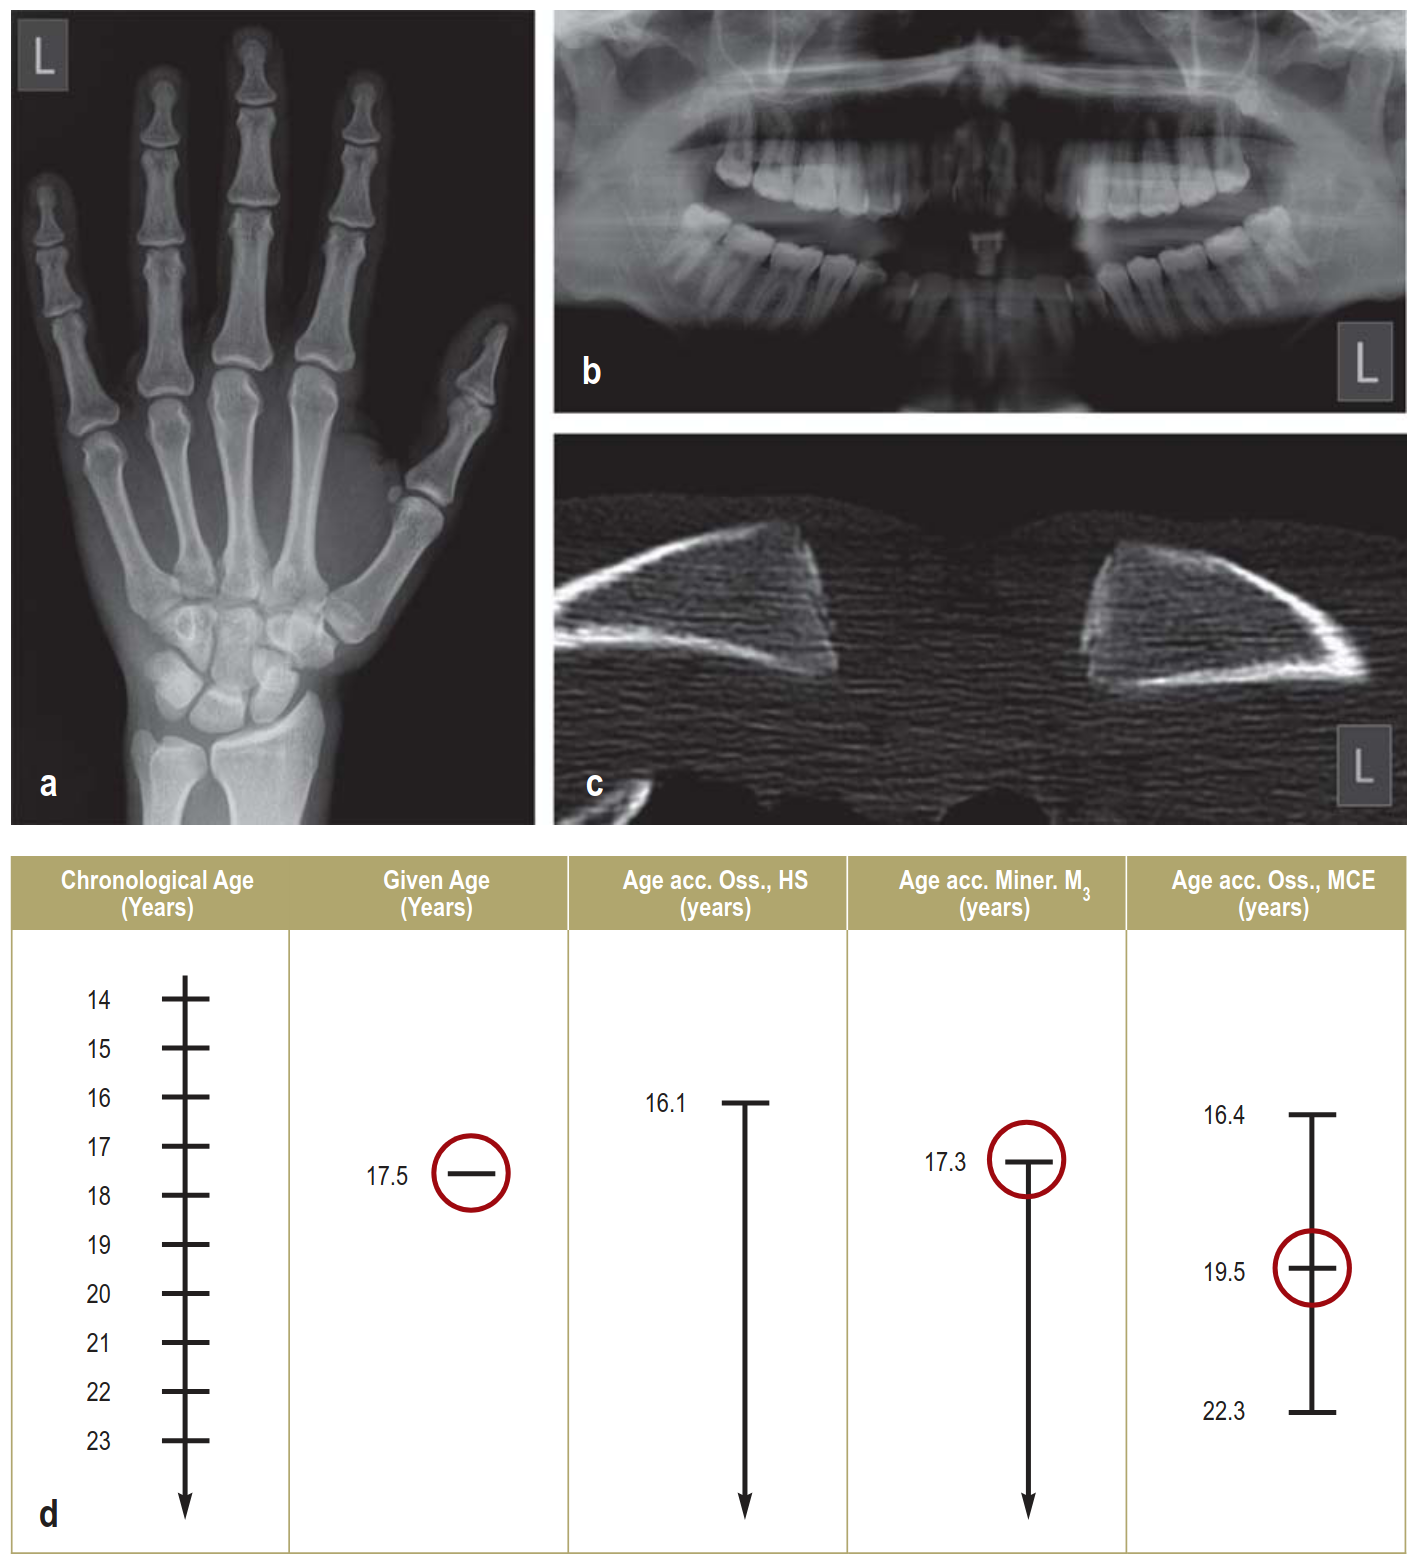
\includegraphics[width=\textwidth]{capitulos/cap_03/imagenes/X_ray_images.png}
    \caption[
        Hallazgos radiológicos en un posible menor con edad disputada: criterio de edad mínima para la determinación de edad. 
        Recuperado de la Figura 1 de \cite{schmeling2016}. 
    ]{
        Hallazgos radiológicos en un posible menor con edad en disputa. Criterio de edad mínima para la determinación de edad. 
        Recuperado de la Figura 1 de \cite{schmeling2016}. 
        El sujeto masculino afirma tener 17,5 años. Tanto la historia clínica como el examen físico no revelan signos de alteraciones en el desarrollo. Se presentan las siguientes imágenes: una radiografía de la mano izquierda en (a), una radiografía panorámica maxilofacial en (b) y una tomografía computarizada de las epífisis mediales de la clavícula en (c). En la imagen (d) se muestran los rangos de edad estimados según los diferentes indicadores radiológicos. Las edades mínimas asociadas a las etapas de desarrollo observadas son 16,1 años, 17,3 años y 16,4 años, respectivamente. La edad mínima del individuo queda determinada por la mayor de estas estimaciones, es decir, 17,3 años. Esta edad mínima estimada es consistente con la edad declarada por el examinado.
    }
    \label{fig:x_ray_images}
\end{figure}

% ------------------------------------------------------------------------------------------------------------

\section{Estimación de la edad en antropología forense usando \textit{machine learning}}

\todo{Incluir gráfica con el número de publicaciones para estimación de la edad en antropología forense usando ML}

Los métodos manuales de estimación del PB se basan en la evaluación visual y en el análisis morfométrico de rasgos esqueléticos. Sin embargo, su aplicación demanda conocimiento especializado, pueden presentar ambigüedades en su formulación que den lugar a interpretaciones variables \cite{berst2001}, y están sujetos a posibles errores de medición \cite{langley2018}, sesgando el proceso y reduciendo su fiabilidad. Estas limitaciones han motivado el desarrollo de métodos automatizados basados en ML, que siguen dos enfoques principales. 

El primero consiste en tomar un método clásico de AF y automatizar sus etapas mediante herramientas computacionales. Para ello, el método debe definir:

\begin{enumerate}
    
    \item cómo extraer las características relevantes de las imágenes médicas, mediante técnicas de procesamiento de imágenes o morfometría tradicional; y

    \item un modelo de clasificación o regresión que opere sobre estas características predefinidas.

\end{enumerate}

La Figura \ref{fig:MRI_pipeline} ilustra un ejemplo de este enfoque. Entre las propuestas destacadas podemos mencionar BoneXpert \cite{thodberg2008}, que empleaba técnicas clásicas de ML y demostró robustez en poblaciones diversas, tanto en origen geográfico como en condiciones clínicas de adquisición de imágenes \cite{van2009, martin2010, thodberg2010}. 

\begin{figure}[h]
    \centering
    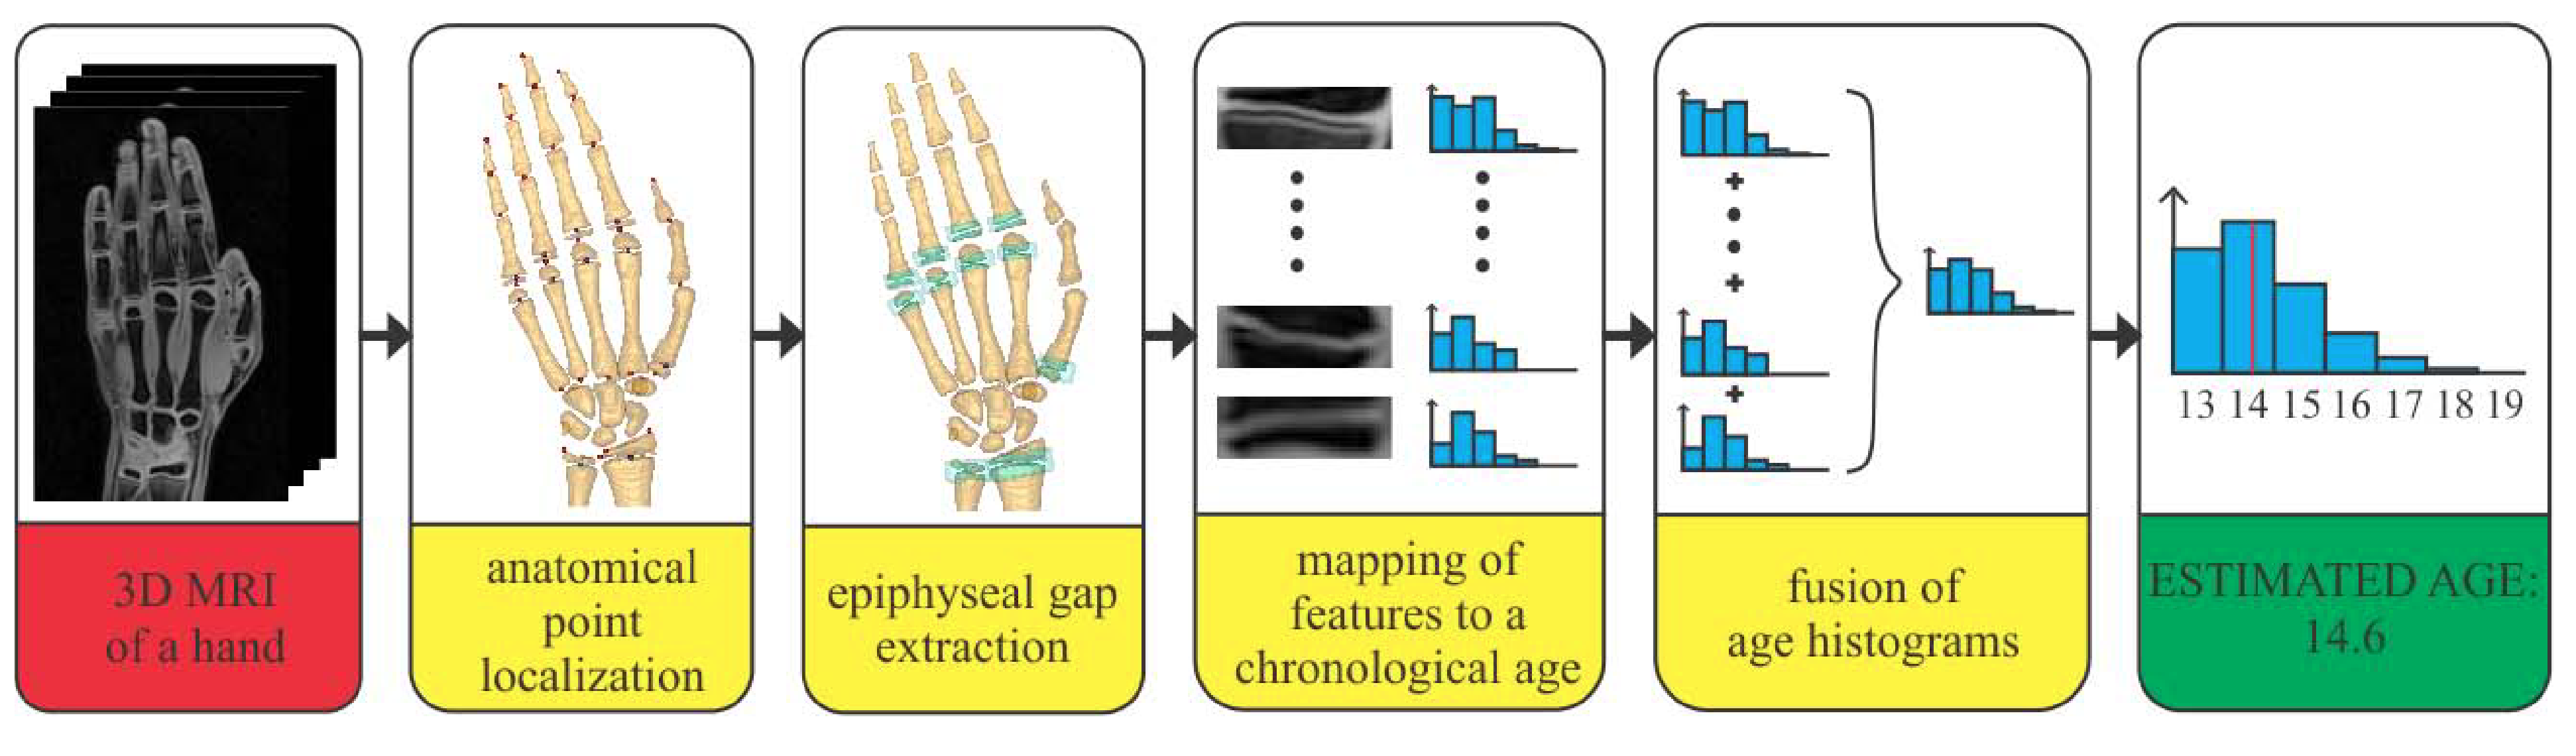
\includegraphics[width=\textwidth]{capitulos/cap_01/imagenes/MRI_pipeline.png}
    \caption[
        Procedimiento secuencial clásico de ML para el método propuesto en \cite{stern2014}.
    ]{
        Procedimiento secuencial clásico de ML para el método propuesto en \cite{stern2014}. 
        Las características se extraen manualmente o con herramientas independientes del modelo.
    }
    \label{fig:MRI_pipeline}
\end{figure}

En cambio, el auge del \textit{deep learning}, impulsó el aprendizaje extremo a extremo (\textit{end-to-end learning}), donde un único modelo aprende de manera automática tanto la extracción de características como la clasificación/regresión a partir de los datos en bruto. Las redes neuronales convolucionales consiguen eliminar la dependencia de criterios antropológicos preestablecidos, y permiten al modelo extraer por sí mismo las características más relevantes para la tarea en que se entrenan. 

\begin{figure}[h]
    \centering
    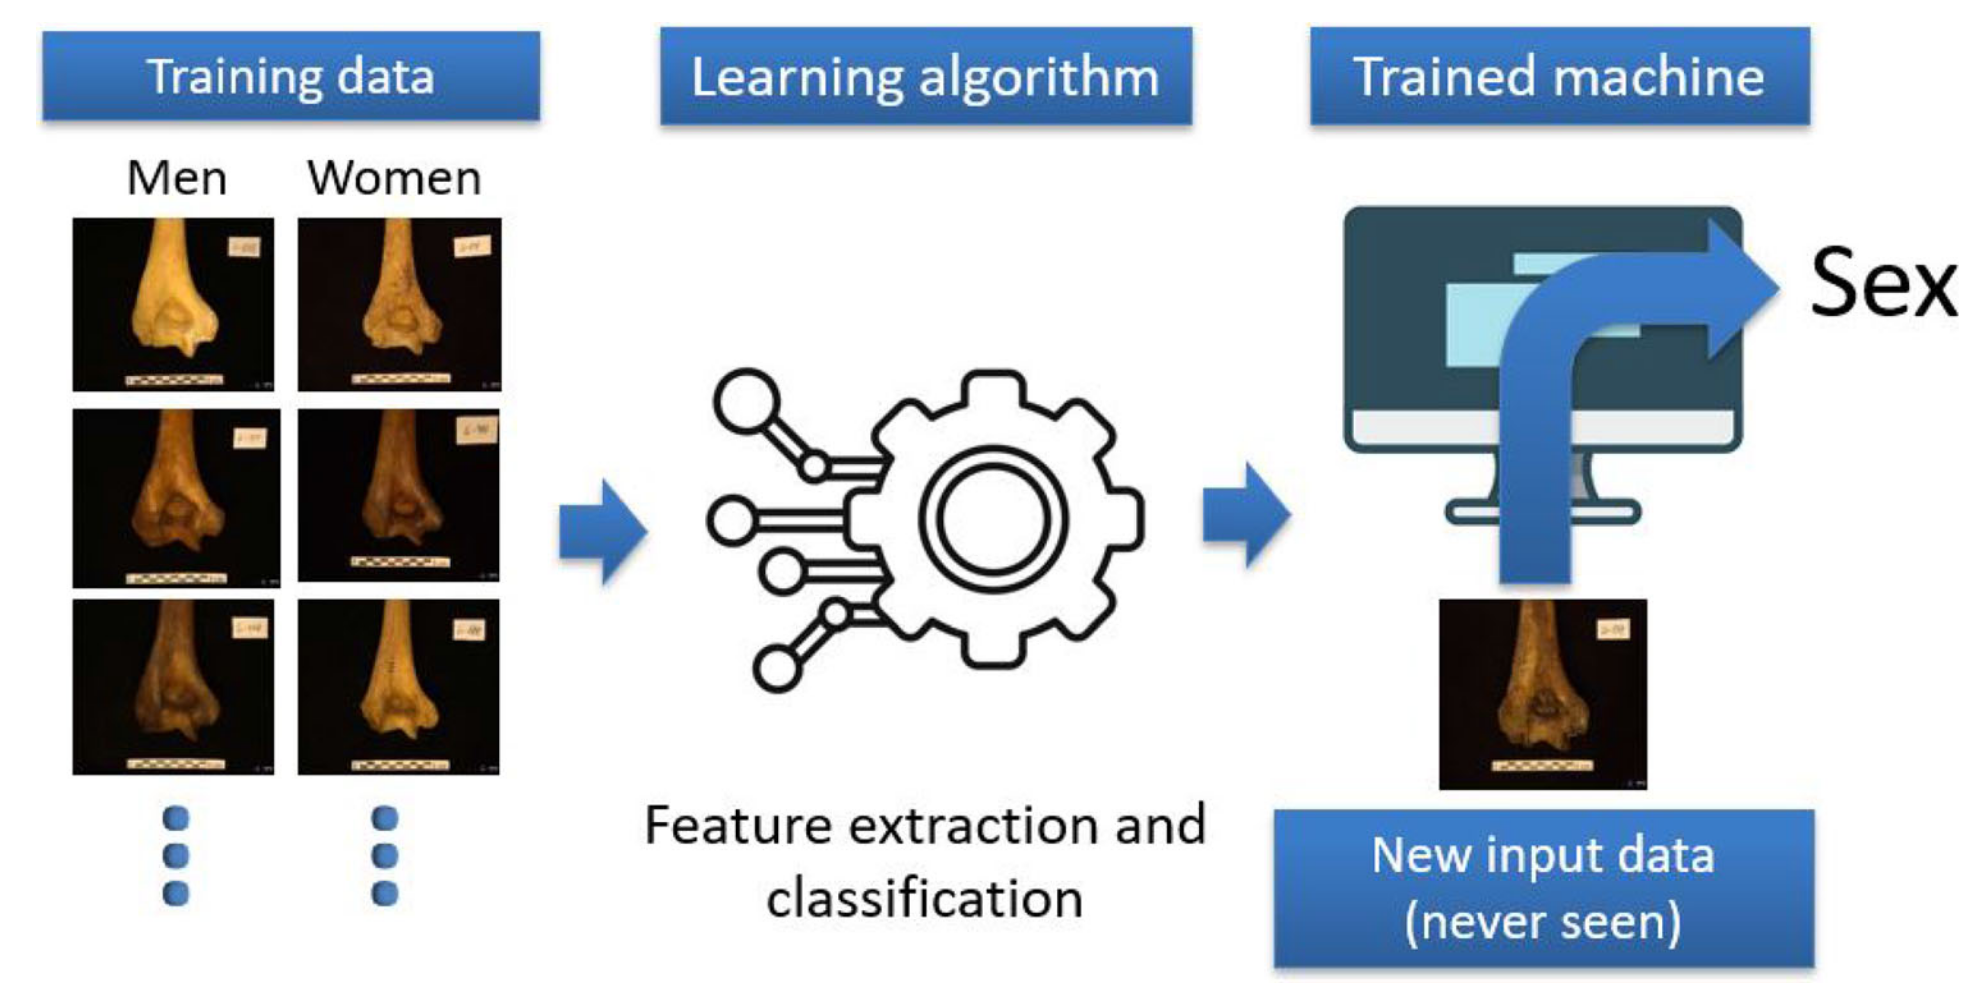
\includegraphics[width=\textwidth]{capitulos/cap_03/imagenes/end-to-end_learning.png}
    \caption[
        Metodología de construcción de un modelo \textit{end-to-end}. 
        Recuperado de \cite{venema2022}.
    ]{
        Metodología de construcción de un modelo \textit{end-to-end}. 
        Recuperado de \cite{venema2022}.
        La CNN aprende a extraer las características de la manera más conveniente para resolver el problema en el que se le entrena, en este caso estimación de sexo.
    }
    \label{fig:end-to-end_model}
\end{figure}

Siguiendo este paradigma, se han propuesto numerosos modelos basados en redes convolucionales. Un ejemplo destacado es el propuesto en \cite{stern2019}, el cual, entrenado con resonancias magnéticas 3D de manos, aprende a identificar las características más relevantes para la estimación de edad automáticamente. Este modelo se ha consolidado como estado del arte en su dominio, alcanzando un error absoluto medio de $0.37 \pm 0.51$ años%
\footnote{
    Esta notación, como veremos a continuación, representa el error absoluto medio y su desviación estándar.
}. 
Además, los autores demostraron su adaptabilidad al procesar imágenes 2D de radiografías, logrando también un rendimiento líder en el ámbito de rayos X.

% ------------------------------------------------------------------------------------------------------------

\section{Cuantificación de la incertidumbre para la estimación de la edad}

\todo{Incluir gráfica con el número de publicaciones para cuantificación de la incertidumbre en estimación de la edad}

La mayoría de trabajos académicos de AF no presentan un enfoque explícito en la cuantificación de incertidumbre de las predicciones, pero sí evalúan la confiabilidad de los métodos propuestos, a través del análisis del error. 

El enfoque principal en la evaluación de estos métodos consiste en comparar la edad cronológica (la \textit{ground truth}) con la edad biológica (la estimada), las cuales no siempre presentan una correlación directa \cite{marquez2015}.

Es por ello que los métodos manuales suelen estimar intervalos de edad o, en casos específicos ---especialmente en contextos legales---, valores de edad mínima probable. Esto se debe a la variabilidad biológica entre individuos, influenciada por factores genéticos, ambientales, nutricionales y de salud, que impide establecer una edad cronológica exacta a partir de los indicadores empleados. En general, los intervalos son determinados en base a una población de referencia, y se suele escoger un intervalo que cubra un 95\% de los casos esperados \cite{garvin2012} (veáse un ejemplo en la Figura \ref{fig:range_values_epiphyselial}).

\begin{figure}[h]
    \centering
    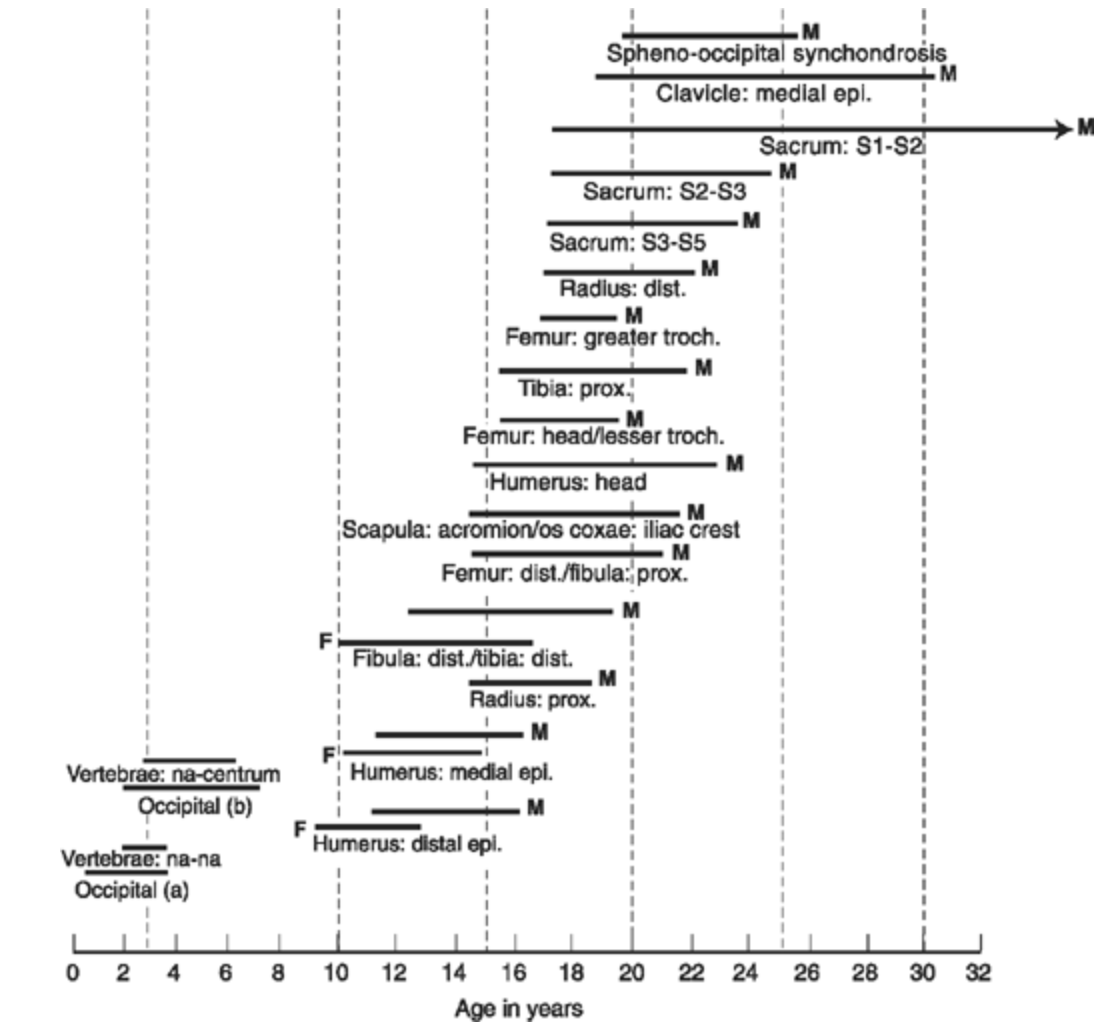
\includegraphics[width=\textwidth]{capitulos/cap_03/imagenes/range_values_epiphyselial.png}
    \caption[
        Cronograma de desarrollo de la unión epifisaria. Recuperado de \cite{byers2023}, original de \cite{buikstra1994}.
    ]{
        Cronograma de desarrollo de la unión epifisaria. Recuperado de \cite{byers2023}, original de \cite{buikstra1994}. 
        Este gráfico combina información de diferentes fuentes sobre los rangos de edades en los que ocurre la fusión de diversas epífisis del esqueleto humano, representado con una línea que indica la variabilidad del momento en que puede producirse dicha fusión con un 95\% de confianza, permitiendo estimar la edad del individuo a partir del grado de unión observado.
    }
    \label{fig:range_values_epiphyselial}
\end{figure}

Por otro lado, los modelos de ML suelen generar predicciones puntuales (valores únicos) sin proporcionar intervalos de confianza o distribuciones probabilísticas asociadas. De esta forma, la edad biológica se trata como una construcción artificial ---cuyos valores son los predichos por el modelo---, que, idealmente, representan las edades cronológicas más probables en un continuo de cambios observado en un dominio concreto, que son generalmente imágenes médicas. 

La métrica más empleada para esta evaluación es el error absoluto medio $\pm$ la desviación estándar. Esta cuantifica el error absoluto promedio entre la edad cronológica y la edad biológica predicha, proporcionando una medida de la precisión del modelo; y la desviación estándar indica la dispersión de estos errores, reflejando la consistencia del modelo en sus predicciones. Otras métricas como el coeficiente de correlación de Pearson ($r$) o el coeficiente de determinación ($R^2$) ---aunque menos frecuentes--- aportan información sobre la relación lineal entre predicciones y valores reales.

Sin embargo, estas métricas pueden esconder sesgos en ciertos grupos etarios%
\footnote{
    Los grupos etarios son intervalos de edad utilizados para clasificar a la población o a los sujetos de estudio en categorías específicas según su edad cronológica.
}, 
y un modelo con mal desempeño en la población general, puede arrojar buenos resultados en algunos grupos específicos, o viceversa. Es por ello que el análisis se puede completar empleando las métricas en subpoblaciones específicas, apoyándose en representaciones gráficas, permiten visualizar las relaciones no lineales entre variables, así como identificar patrones, tendencias o valores atípicos. Entre ellas destacan: 

\begin{itemize}

    \item Gráficas de dispersión: comparando edad cronológica vs. edad biológica, o mostrando errores en función de las edades cronológica o biológica (véase la Figura \ref{fig:error_distribution_by_age}).

    \item Histogramas, gráficos de densidad o diagramas de cajas para representar la distribución de errores. En la Figura \ref{fig:error_study_stern2019} vemos un ejemplo en el que plasman un histograma escrito como texto.

\end{itemize}

\begin{figure}[h]
    \centering
    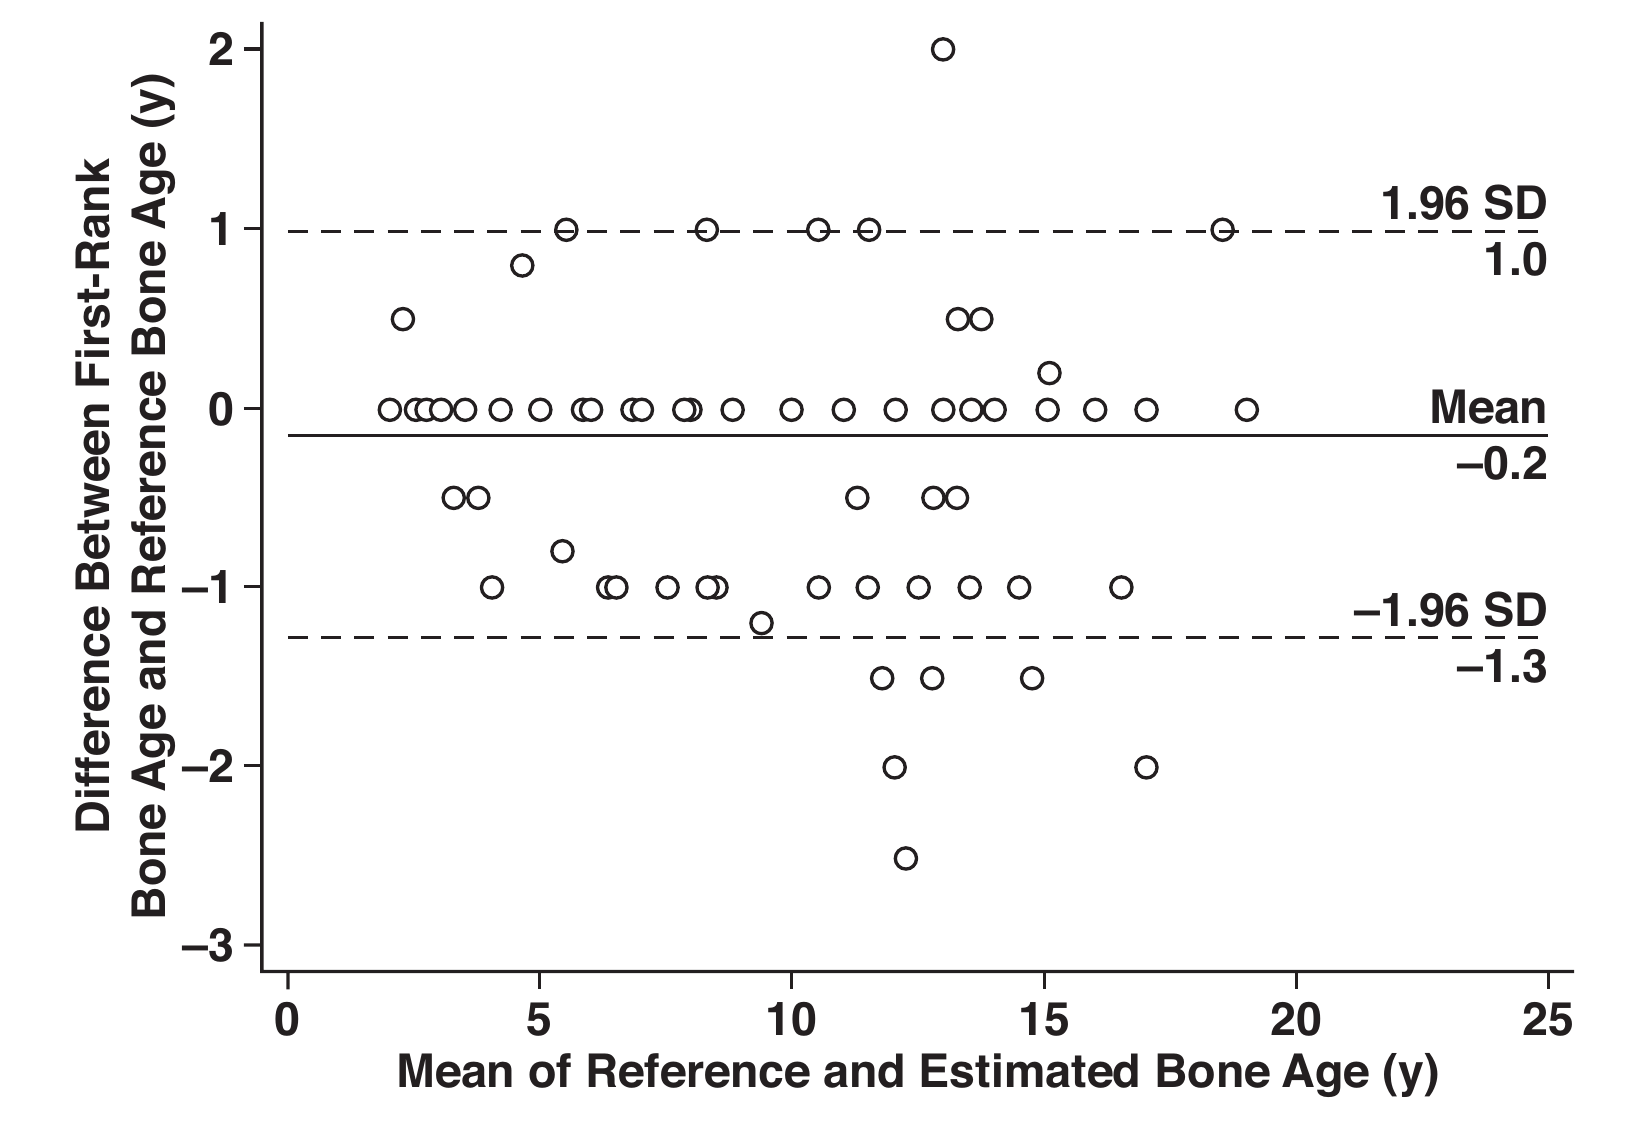
\includegraphics[width=0.8\textwidth]{capitulos/cap_03/imagenes/error_distribution.png}
    \caption[
        Distribución del error por edad real para el modelo propuesto en \cite{kim2017}. 
    ]{
        Distribución del error por edad real para el modelo propuesto en \cite{kim2017}. 
        Recuperado de la Figura 3.  
        Esta visualización permite observar el error en cada instancia predicha para diferentes edades reales. 
    }
    \label{fig:error_distribution_by_age}
\end{figure}

\begin{figure}[h]
    \centering
    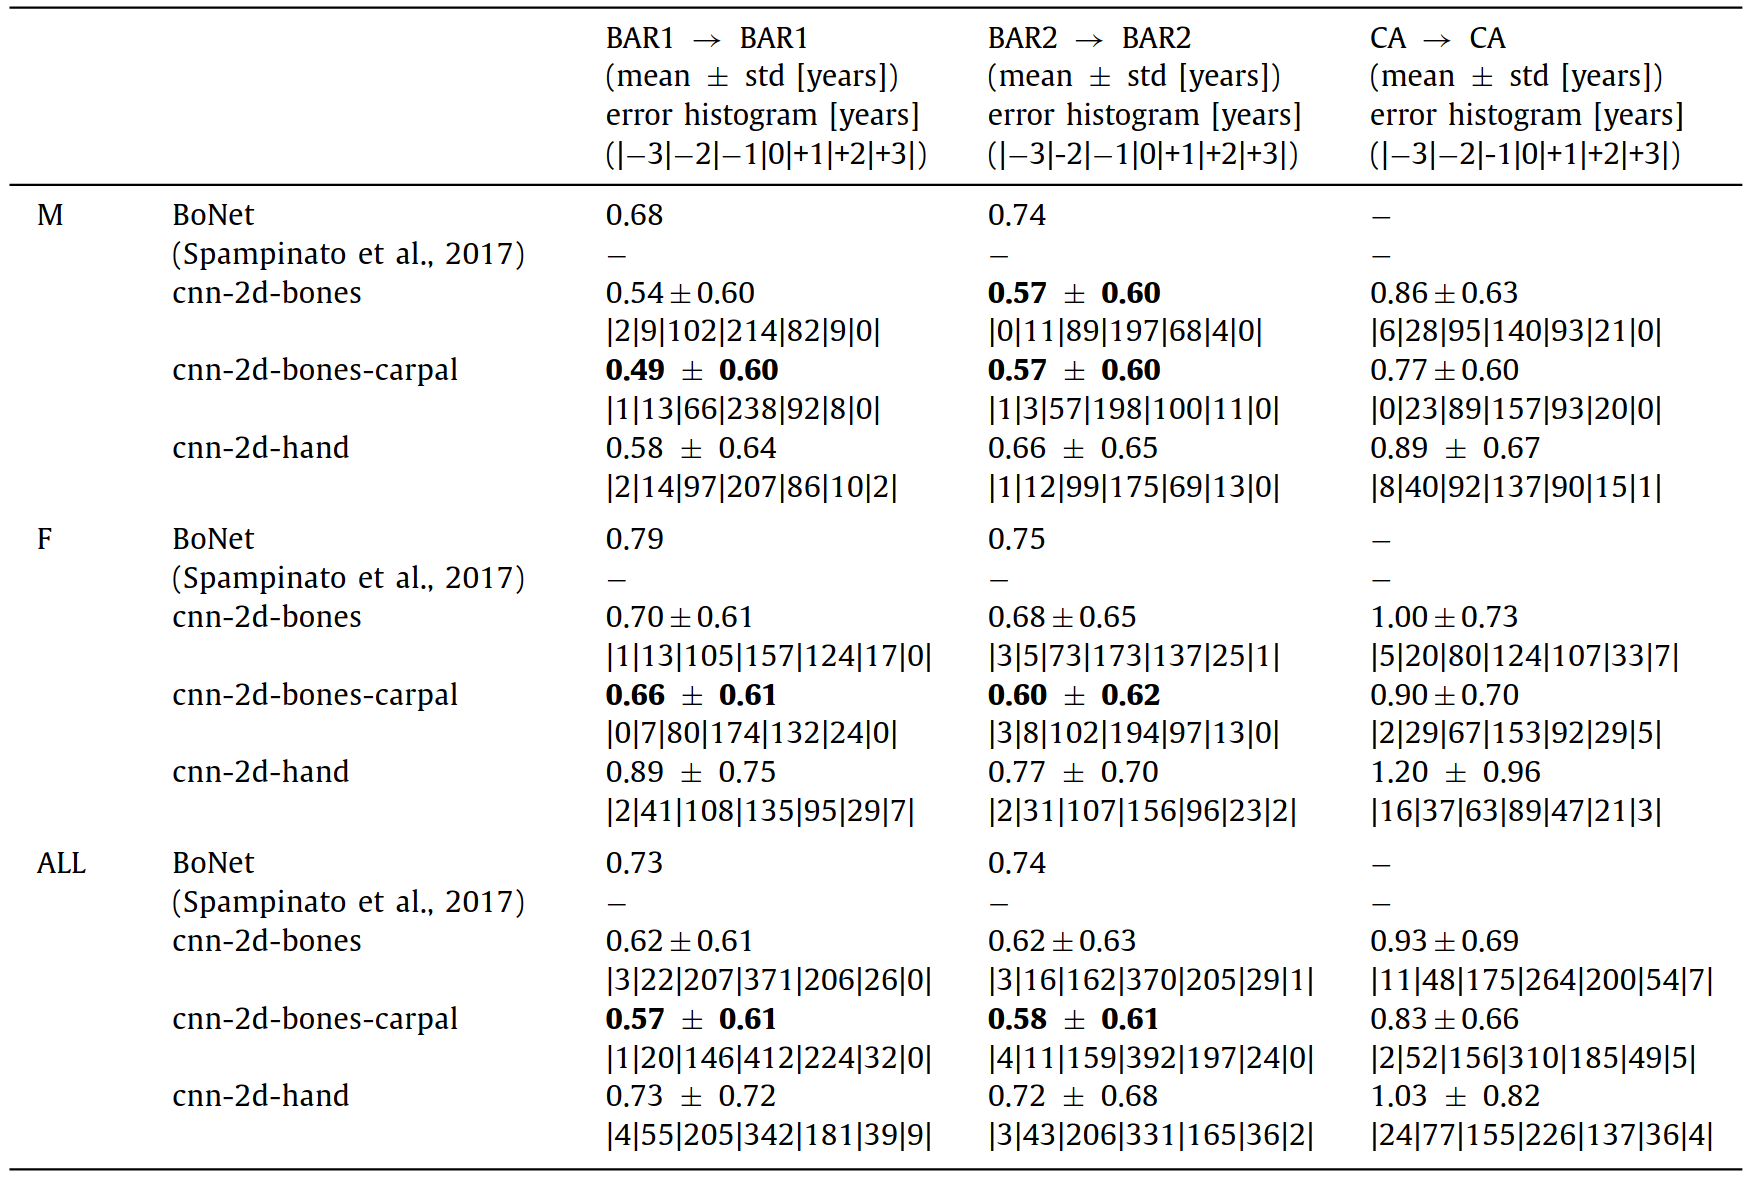
\includegraphics[width=\textwidth]{capitulos/cap_03/imagenes/error_study.png}
    \caption[
        Estudio del error en los métodos 2D propuestos en \cite{stern2019}.
    ]{
        Estudio del error en los métodos 2D propuestos en \cite{stern2019}. 
        Recuperado de la Tabla 2 de \cite{stern2019}. 
        Se observa que se muestra tanto el error absoluto medio $\pm$ desviación estándar como un histograma de errores, que permite ver la distribución general de los errores. 
    }
    \label{fig:error_study_stern2019}
\end{figure}


% ------------------------------------------------------------------------------------------------------------

\section{Estimación del sexo en antropología forense}

% ------------------------------------------------------------------------------------------------------------


% \section{Predicción conformal}





% \begin{itemize}

%     \item La media del error absoluto medio $\pm$ desviación estándar: Esta métrica cuantifica el error 
%     absoluto promedio entre la edad cronológica y la edad biológica predicha, proporcionando una medida 
%     de la precisión del modelo. La desviación estándar indica la dispersión de estos errores, reflejando la 
%     consistencia del modelo en sus predicciones.

%     \item El \textit{P value}


    
%     \item La raíz del error cuadrático medio: 
    
%     \todo{¿Se ve bien que yo hable aquí de métricas y vuelva a hacerlo más a fondo en el apartado 5? ¿O tal
%     vez debería introducir las métricas en Fundamentos teóricos?}
    
%     \item Gráficos de dispersión de edad cronológica vs edad biológica: Permiten visualizar la relación 
%     entre las edades reales y las predichas, así como identificar patrones, tendencias o valores atípicos.
    
%     \item Ratio de concordancia: Definido como la proporción de casos para los cuales la edad estimada y la 
%     real concuerdan

%     \item Coeficiente de correlación de Pearson ($r$): Este evalúa la relación lineal entre las edades 
%     cronológicas y las predichas. Un valor cercano a 1 indica una fuerte correlación positiva, lo que 
%     sugiere que el modelo predice correctamente la tendencia en los datos.


% \end{itemize}


% Las previas para grupos concretos

% Sin embargo, ...
% existe variabilidad inherente en la correspondencia entre edad biológica y cronológica, porque dos personas
% con la misma edad cronológica pueden presentar edades biológicas significativamente diferentes 









% Fenómeno que ocurre: se trata la estimación de edad como una clasificación, y se evalúa como tal.
% Problema: Se está creando una distancia artificial entre instancias de edades muy cercanas pero distintos enteros.

